\documentclass[aspectratio=43]{beamer}

\graphicspath{{../figures/}{./}}

\usepackage{cmap}
\usepackage[T2A]{fontenc}
\usepackage[utf8]{inputenc}
\usepackage[russian]{babel}
\usepackage{ragged2e}
\usepackage{tikz}
\usetikzlibrary{positioning}
\usepackage{array}
\usepackage{multicol}
\usepackage{booktabs}
\usepackage{csquotes}
\usepackage{amssymb,amsfonts,amsmath}

\usecolortheme{beaver}
\usefonttheme[onlymath]{serif}
\setbeamertemplate{navigation symbols}{}
\setbeamertemplate{footline}[page number]
\setbeamertemplate{blocks}[default]
\setbeamercolor{block title}{fg=black,bg=black!15}
\setbeamercolor{block body}{fg=black,bg=black!6}
\setbeamersize{text margin left=0.5cm,text margin right=0.5cm}
\setbeamerfont{author}{size=\normalsize}
\setbeamerfont{institute}{size=\normalsize}
\setbeamerfont{date}{size=\normalsize}
\setbeamerfont{frametitle}{series=\bfseries}
\setbeamertemplate{enumerate item}{\insertenumlabel.}
\setbeamertemplate{enumerate subitem}{\insertenumlabel.}

\newtheorem{rustheorem}{Теорема}
\newtheorem{rusdefinition}{Определение}
\newtheorem{ruscorollary}{Следствие}

%----------------------------------------------------------------------------------------------------------
\title[Геометрический подход к оценке сложности данных]
{Геометрический подход к оценке сложности данных\\ на основе генеративных диффузионных моделей}
\author[Д.\,В.~Черноусов]{\large Черноусов Данила Владиславович}
\institute{\large
Московский физико-технический институт\\
~\\
\footnotesize{03.03.01 Прикладные математика и физика\\
~\\
Научный руководитель к.ф.-м.н. А.\,В.~Грабовой}
}
\date{\footnotesize{МФТИ, г. Долгопрудный\\ 2026 г.}}
%----------------------------------------------------------------------------------------------------------

\begin{document}

% ============================================================
% Слайд 1: Титульный лист
% ============================================================
\begin{frame}
\titlepage
\end{frame}

% ============================================================
% Слайд 2: Актуальность
% ============================================================
\begin{frame}{Актуальность}
    \textbf{Зачем измерять сложность данных:}
    \begin{itemize}
        \item \textbf{Интерпретируемость} --- предсказание качества модели
              по характеристикам обучающей выборки, а не только по её размеру
        \item \textbf{Адаптивное обучение} --- обучающие батчи с учётом сложности данных
        \item \textbf{Оценка разнообразия} --- сравнение выборок одного размера,
              но разного содержания
    \end{itemize}
\end{frame}

% ============================================================
% Слайд 3: Постановка задачи
% ============================================================
\begin{frame}{Постановка задачи}
\justifying

\textbf{Исследуемая проблема}

Построение интерпретируемой меры сложности выборки данных, согласованной с
геометрией порождающего распределения.

~\\
\textbf{Задачи}

\begin{enumerate}
\justifying
    \item Исследовать достаточные условия корректности меры сложности выборки.
    \item Предложить метод оценки сложности выборки, учитывающий семантическую
          структуру данных.
\end{enumerate}

~\\
\textbf{Метод}

Сложность выборки строится по симметричному ядру на парах объектов. Мера
определяется через матрицу этого ядра, корректность вытекает из достаточных условий. Ядро строится по предобученной диффузионной модели. Объекту сопоставляется его траектория порождающего процесса, описывающая объект
сразу на всех масштабах.
\end{frame}

% ============================================================
% Слайд 4: Что такое мера сложности
% ============================================================
\begin{frame}{Определение меры сложности}
\justifying

Выборка $X = (x_1, \dots, x_N)$, \;$x_i \in \mathbb{R}^d$,

\medskip
\begin{rusdefinition}
\emph{Мерой сложности} назовём отображение $\mu_D(X) \in \mathbb{R}_+$,
удовлетворяющее трём свойствам:
\begin{enumerate}
    \item \textbf{Инвариантность к перестановкам:}\;
          $\mu_D(\pi X) = \mu_D(X)$, \;$\pi \in S_N$;
    \item \textbf{Субаддитивность:}\;
          $\mu_D(X \cup Y) \le \mu_D(X) + \mu_D(Y)$;
    \item \textbf{Монотонность:}\;
          $\mu_D(X) \le \mu_D(X \cup \{x\})$.
\end{enumerate}
\end{rusdefinition}
\end{frame}

% ============================================================
% Слайд 5: Достаточное условие корректности
% ============================================================
\begin{frame}{Достаточное условие корректности}
\justifying

Зададим симметричное ядро $k(x, y)$ на парах объектов и
построим по его матрице $K = \bigl(k(x_i, x_j)\bigr)$ меру сложности
\[
    \mu_D(X) = \log\det\bigl(I + K\bigr).
\]

\begin{rustheorem}[Черноусов, 2026]
Пусть ядро $k$ положительно полуопределено ($K \succeq 0$) и
$k(x,x) = 1$ для любого $x$. Тогда $\mu_D(X) = \log\det(I+K)$~--- мера
сложности: выполнены свойства (1)--(3).
\end{rustheorem}
\end{frame}

% ============================================================
% Слайд 6: Границы на возрастание сложности
% ============================================================
\begin{frame}{Границы на возрастание сложности}
\begin{rustheorem}[Черноусов, 2026]
Пусть ядро $k$ положительно полуопределено, $k(x,x)=1$ для любого $x$. Тогда для
любой выборки $X$ объёма $N$ и объекта $x$
\[
    \log\tfrac{N+2}{N+1} \le \mu_D(X\cup\{x\}) - \mu_D(X) \le \log 2.
\]
\end{rustheorem}
\begin{ruscorollary}
$\log(N{+}1) \le \mu_D(X) \le N\log 2$, \;$N = |X|$.
\end{ruscorollary}
\end{frame}

% ============================================================
% Слайд 7: Метрика в пространстве объектов
% ============================================================
\begin{frame}{Метрика в пространстве объектов}
\justifying

\begin{rustheorem}[Черноусов, 2026]
Пусть $(T,w)$~--- пространство с мерой, $p\in(0,2]$, $\beta\in(0,2]$,
$\lambda>0$, и отображение $x\mapsto\varphi_x\in L^p(T,w;\mathbb{R}^d)$
инъективно. Тогда
\[
    D(x,y)=\Big(\int_T\|\varphi_x(t)-\varphi_y(t)\|^{p}\, w(t)\,dt\Big)^{1/2}
\]
--- метрика, а ядро $k(x,y)=e^{-\lambda\,D(x,y)^{\beta}}$ положительно
полуопределено.
\end{rustheorem}

\begin{center}
$\beta=2$:\, гауссово $e^{-\lambda D^2}$;\qquad
$\beta=1$:\, лапласово $e^{-\lambda D}$.
\end{center}
\end{frame}

% ============================================================
% Слайд 8: Диффузионный процесс и поток вероятности
% ============================================================
\begin{frame}{Диффузионный процесс и поток вероятности}
\justifying

Обозначим за $p$ плотность распределения данных, а тогда \textbf{зашумление} и
\textbf{скор-функция}:
\[
    p_t = p * \mathcal{N}\bigl(0, \sigma^2(t) I\bigr),
    \qquad
    s(x,t) = \nabla_x \log p_t(x).
\]

\smallskip
Стохастическому процессу зашумления соответствует детерминированное \textbf{ОДУ
вероятностного потока} с теми же маргинальными плотностями $p_t$ при каждом $t$:
\[
    \tfrac{dz}{dt} = -\dot\sigma\,\sigma\, s(z,t),\qquad z(0)=x.
\]
Объект идёт по единственной траектории от данных к шуму.

\medskip
Траектория проходит все уровни шума и на разных масштабах кодирует разную
близость объектов:
\begin{columns}[T]
\begin{column}{0.5\textwidth}
\begin{itemize}
    \item малый шум ($t\to0$): \textbf{синтаксис} (форма, внешний вид);
\end{itemize}
\end{column}
\begin{column}{0.5\textwidth}
\begin{itemize}
    \item большой шум ($t\to1$): \textbf{семантика} (класс, смысл).
\end{itemize}
\end{column}
\end{columns}

\medskip
{\footnotesize Истинный скор $\nabla_x\log p_t$ неизвестен, его оценивает
обученная диффузионная модель $s_\theta \approx \nabla_x\log p_t$.}
\end{frame}

% ============================================================
% Слайд 9: Предлагаемый метод — траекторное вложение
% ============================================================
\begin{frame}{Предлагаемый метод: траекторное вложение}

\noindent\makebox[\linewidth]{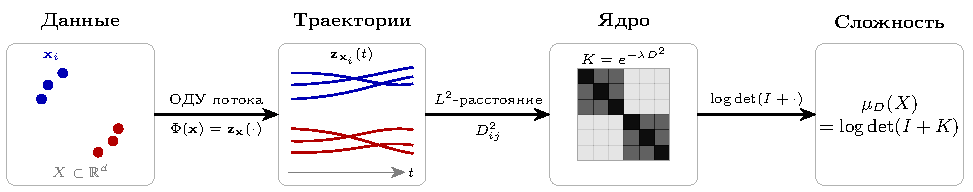
\includegraphics[width=\dimexpr\paperwidth-4mm\relax]{principle.pdf}}

\justifying
\medskip
\textbf{Вложение} $\Phi(x) = z_x(\cdot) \in \mathcal{H} = L^2\bigl([0,1], \mu_w; \mathbb{R}^d\bigr)$:
объект описан всей траекторией, на всех уровнях шума. Расстояние с весом
$w(t)=\mathrm{Beta}(t;a,b)$:
\[
    D^2(x_i, x_j) = \int_0^1 \|z_{x_i}(t) - z_{x_j}(t)\|^2\,
    \underbrace{w(t)}_{\text{вес масштаба}}\, dt.
\]

\begin{center}
\setlength{\fboxsep}{6pt}
\fbox{$\displaystyle \mu_D(X) = \log\det\Big(I + \Big(e^{-\lambda \int_0^1 \|z_{x_i}(t)-z_{x_j}(t)\|^2 w(t)\,dt}\Big)_{i,j=1}^N\Big)$}
\end{center}
\end{frame}

% ============================================================
% Слайд 10: Эксперимент 1: скорость роста
% ============================================================
\begin{frame}{Эксперимент 1: скорость роста}
    \begin{columns}[T]
        \begin{column}{0.55\textwidth}
            \begin{figure}
                \centering
                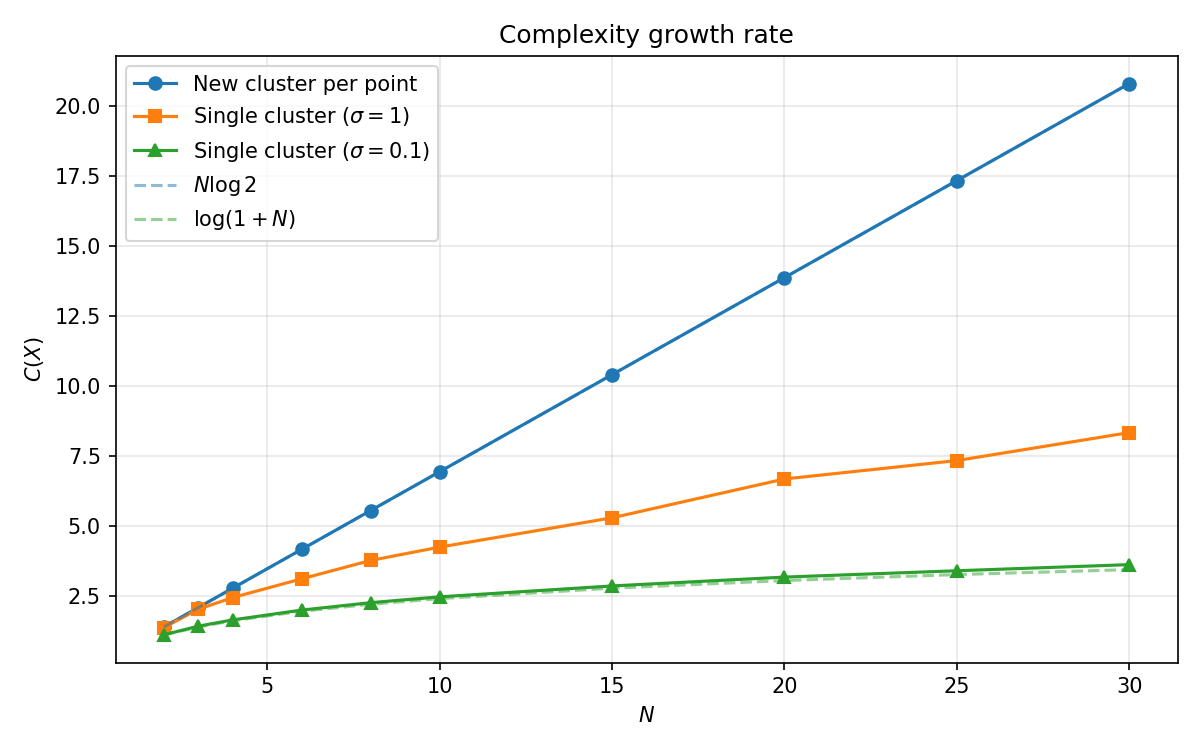
\includegraphics[width=\textwidth]{growth_rate.png}
            \end{figure}
        \end{column}
        \begin{column}{0.42\textwidth}
            \medskip
            Синтетическая смесь гауссиан, $d = 2$, аналитическая скор-функция.

            \bigskip
            \begin{itemize}
                \item $N$ кластеров по 1 точке: $\mu_D \approx N\log 2$;
                \item один кластер, $\sigma = 0.1$: $\mu_D \approx \log(1+N)$;
                \item один кластер, $\sigma = 1$: промежуточный рост.
            \end{itemize}
        \end{column}
    \end{columns}
\end{frame}

% ============================================================
% Слайд 11: Эксперимент 2: MNIST
% ============================================================
\begin{frame}{Эксперимент 2: MNIST}
    \begin{columns}[T]
        \begin{column}{0.55\textwidth}
            \begin{figure}
                \centering
                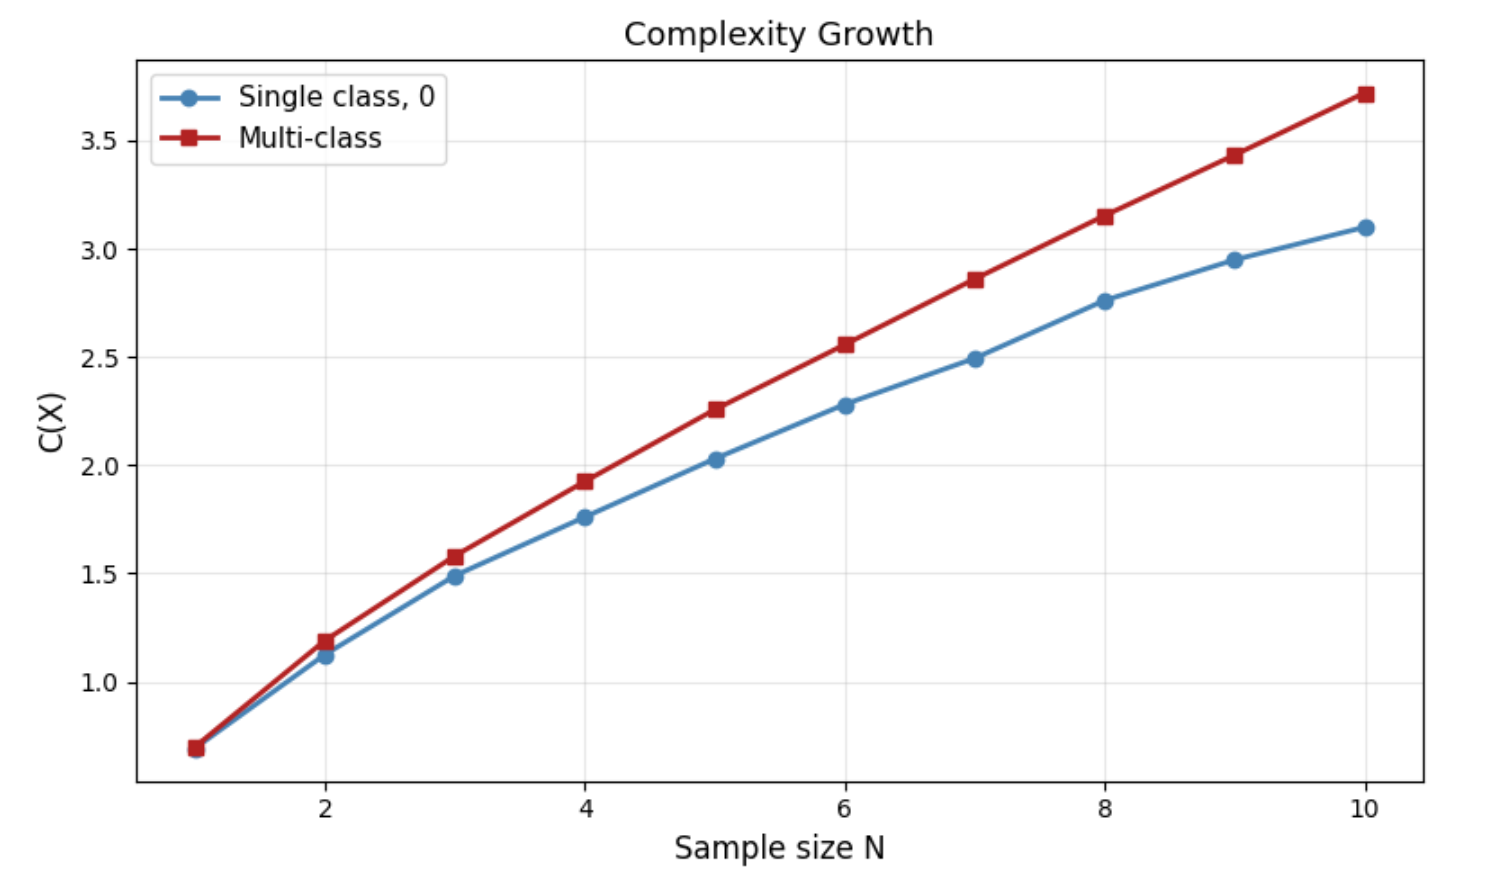
\includegraphics[width=\textwidth]{Mnist_picture.png}
            \end{figure}
        \end{column}
        \begin{column}{0.42\textwidth}
            \medskip
            Предобученная DDPM, ОДУ вероятностного потока.

            \bigskip
            \begin{itemize}
                \item один класс vs несколько классов;
                \item $\mu_D$ мультикласса растёт быстрее;
                \item разнообразные данные $\rightarrow$ большая сложность.
            \end{itemize}
        \end{column}
    \end{columns}
\end{frame}

% ============================================================
% Слайд 12: Выносится на защиту
% ============================================================
\begin{frame}{Выносится на защиту}
\justifying
\begin{enumerate}
    \item Доказана теорема о достаточном условии корректности меры сложности
          выборки.
    \item Доказана теорема о свойствах предложенной меры.
    \item Предложен метод оценки сложности на основе траекторного вложения
          диффузионной модели.
    \item Экспериментально подтверждена семантическая согласованность
          предложенной меры.
\end{enumerate}

\bigskip
\textbf{Работы автора по теме ВКР}
\begin{itemize}
    \item Основные результаты доложены на 68-й Всероссийской научной конференции
          МФТИ.
    \item По теме работы подготовлена статья, поданная на конференцию
          ICOMP~2026.
\end{itemize}
\end{frame}

% ============================================================
% Слайд 13: Список литературы  (НУЖЕН ЛИ? — см. вопрос)
% ============================================================
% \begin{frame}{Список литературы}
% \end{frame}

\end{document}
